\section{Basics}


\subsection{Default Parameterization}

From the user's point of view, this package's basic entry point is:

\ccFunction{Parametizer_traits_3<MeshAdaptor_3>::Error_code parameterize (MeshAdaptor_3 * mesh);}
{
Compute a 1 to 1 mapping from a triangular 3D surface 'mesh' to 2D circle, using
Floater's mean value coordinates algorithm. 1 to 1 mapping is guaranteed.
The mapping is linear by pieces (linear in each triangle). The result is the (u,v) pair image of each vertex of the 3D surface.
Preconditions:\begin{itemize}
\item 'mesh' must be a surface with 1 connected component.\item 'mesh' must be a triangular mesh.\item the mesh border must be mapped onto a convex polygon.\end{itemize}
}
\begin{description}
\item[Parameters: ]
\begin{description}
\item[mesh]3D mesh, model of MeshAdaptor\_3 concept \end{description}
\end{description}

This CGAL::parameterize() function provides a default parameterization method: Floater's
mean coordinate values, with an arc length circular border parameterization, and using
OpenNL sparse linear solver.

The result is stored in the (u,v) fields of the mesh's vertices and/or halfedges.

% Include floater.png/eps figure with title = "Floater's mean value coordinates parameterization"
\begin{figure}[bht]
    \begin{center}
        % Image
        \begin{ccTexOnly}
            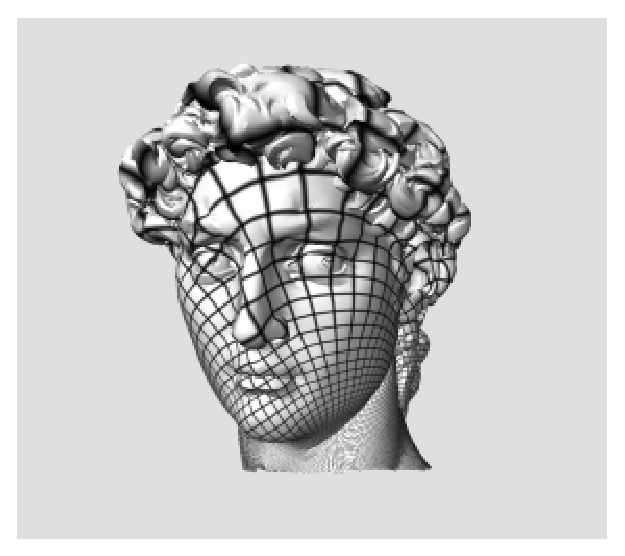
\includegraphics{Parameterization/floater} % omit suffix to support PS and PDF
        \end{ccTexOnly}
        \begin{ccHtmlOnly}
            <img border=0 src="./floater.png" align=center>
        \end{ccHtmlOnly}
        \label{parameterization-fig-floater}

        % Title
        \caption{Floater's mean value coordinates parameterization}
    \end{center}
\end{figure}


\subsection{Supported Meshes List and Concept}

The general definition of input meshes handled by the package is:

\begin{itemize}

\item Triangulated

\item 2-manifold

\item Oriented.

\item The input mesh can be of any genus and have any number of connected components,
-but- it has to come with a description of a boundary (a list of
vertices) which is the boundary of
a topological disc. If no boundary is given, we assume that it
coincides with the longest boundary already in the input mesh.

Note that this way the user is responsible for cutting a closed mesh of
arbitrary genus (even a topological disc with an intricate seam
cut), as long as this condition is verified.

The package will only parameterize the inside part of the given boundary,
thus only one connected component.

\end{itemize}

The package accesses such meshes through the MeshAdaptor\_3 concept. Among other
things, this concept defines the accessor to the (u,v) values computed
by parameterizations.

The package proposes
a MeshAdaptor\_3 interface with both the 2D Triangulation Data Structure enriched
with 3D points (not yet implemented) and the Polyhedron:

\ccRefIdfierPage{CGAL::Mesh_adaptor_polyhedron_3}  \\

Note that these interfaces are decorators that add "on the fly" the necessary
fields to unmodified CGAL data structures (using STL maps).
For performance reasons, it is recommended to use CGAL data structures
enriched with the proper fields.
See Polyhedron\_ex class in polyhedron\_ex\_parameterization.C example.


\subsection{Default Parameterization Example}

The code below applies the default parameterization to a Polyhedron\_3 mesh:

\begin{ccExampleCode}

// CGAL kernel
typedef CGAL::Cartesian<double>                             Kernel;

// Mesh true type and parameterization adaptors
typedef CGAL::Polyhedron_3<Kernel>                          Polyhedron;
typedef CGAL::Mesh_adaptor_polyhedron_3<Polyhedron>         Mesh_adaptor_polyhedron;

// Defines the error codes
typedef CGAL::Parametizer_traits_3<Mesh_adaptor_polyhedron> Parametizer;

int main(int argc,char * argv[])
{
    Polyhedron mesh;
    ...

    // The parameterization package needs an adaptor to handle Polyhedron_3 meshes
    // Note: parameterization methods support only meshes that are toplogical disks
    Mesh_adaptor_polyhedron mesh_adaptor(&mesh);

    // Floater's mean value coordinates parameterization
    Parametizer::Error_code err = CGAL::parameterize(&mesh_adaptor);
    ...
}

\end{ccExampleCode}

See the complete code in Polyhedron\_parameterization1.C example.


